% !TEX program = xelatex
\documentclass[a4paper]{exam}
\usepackage{amsmath}
\usepackage{amsthm}
\usepackage[left=1.8cm,right=1.8cm,top=2.2cm,bottom=2.0cm]{geometry}
\usepackage[UTF8]{ctex}
\usepackage{enumerate}
\usepackage{fancyhdr}
\usepackage{xpatch}
\usepackage{graphicx} 
\usepackage{float} 
\usepackage{subfigure} 
\usepackage{amsfonts}
\usepackage{mathtools}
\usepackage{framed}
\usepackage{multicol}
\usepackage{minted}
\usepackage{fontspec}
\usepackage{float}
\usepackage{tikz}
\usepackage{multicol,comment}
\usepackage{hyperref}
\usepackage{biblatex}
\addbibresource{06-discussion.bib}
\usepackage{tikz}

\usetikzlibrary{automata,positioning}
\theoremstyle{definition}
\newtheorem*{solution*}{\textbf{Solution:}}
\newtheorem*{proof*}{\textbf{Proof:}}
\newtheorem{theorem}{Theorem}[subsection]
\newtheorem{definition}{Definition}[subsection]
\newtheorem{lemma}{Lemma}[subsection]
\makeatletter

\AtBeginDocument{\xpatchcmd{\@thm}{\thm@headpunct{.}}{\thm@headpunct{}}{}{}}
\makeatother
\noprintanswers
\pagestyle{fancy}
\renewcommand{\baselinestretch}{1.15}

\usepackage{paralist}
\let\itemize\compactitem
\let\enditemize\endcompactitem
\let\enumerate\compactenum
\let\endenumerate\endcompactenum
\let\description\compactdesc
\let\enddescription\endcompactdesc

% shorten footnote rule
\xpatchcmd\footnoterule
  {.4\columnwidth}
  {1in}
  {}{\fail}

\title{CS 131 Compilers: Discussion 6: More on Modern Intermediate Representation}
\author{\textbf{杨易为}~~\textbf{吴凌云}~~\textbf{樊雨鑫} \\ \texttt{ \{yangyw,wuly2,fanyx\}@shanghaitech.edu.cn}}

\begin{document}
\maketitle
\section{Object Oriented Programming}
Recall the $stub$ trick from the lecture, an implementation strategy for multiple inheritance is listed as following:

\begin{minted}[mathescape, linenos]{c++}
class Base {
  public:
    int foo;
    virtual int f() {
      std::cout << this << std::endl; 
      return this->foo;
    }
};

class Base2 {
  public:
     int bar;
     virtual int g() {
      std::cout << this << std::endl; 
      return this->bar;
     }
};

class Derived : public Base, public Base2 {
  public:
     int baz;
     virtual int h() {
       std::cout << this << std::endl; 
       return this->baz;
     }
};
\end{minted}

To overcome this issue, compilers will move the this pointer so that each method sees what it expects. For simplicity, they actually create stub methods that will move the this pointer before calling the original method. For example, the compiler may generate

\begin{minted}[mathescape, linenos]{c++}
  Base2::g’() { move_this_pointer(); g(); }
\end{minted}

\begin{enumerate}
  \item Roughly sketch the class layout of the above classes (using the same 4-byte offset convention from the inheritance lecture). For Derived, \texttt{assumeh()} is stored inside its own version of Base’s vtable.
  \begin{solution}
\begin{verbatim}
0 | (Base vtable pointer; vtable contains f())
4 | int foo

0 | (Base2 vtable pointer; vtable contains g())
4 | int bar

0 | (Base vtable pointer; vtable contains f(), h(), and g'(); 
    g'() is a stub that increments this by 8, then calls g())
4 | int bar
8 | (Base2 vtable pointer; vtable contains g())
12| int bar
16| int baz
\end{verbatim}
  \end{solution}
 \item What will the following print (assuming there is no padding)?
\begin{minted}[mathescape, linenos]{c++}
    Derived a;
    std::cout << &a << std::endl; // Suppose this prints 0x10
    a.f();
    a.g();
    a.h();
\end{minted}
\begin{solution}
\begin{verbatim}
0x10
0x18
0x10
\end{verbatim}
\end{solution}
\end{enumerate}
\subsubsection{C++ OOP implementation in LLVM IR\cite{llvmcpp}}
A class is nothing more than a structure with an associated set of functions that take an implicit first parameter, namely a pointer to the structure. Therefore, is is very trivial to map a class to LLVM IR:
\begin{minted}[mathescape, linenos]{c++}
#include<stddef.h>
class Foo {
public:
  Foo() {
      length = 0;
  }

  size_t GetLength() const {
      return length;
  }

  void SetLength(size_t value) {
      length = value;
  }

private:
    size_t length;
};
\end{minted}
We first transform this code into two separate pieces:
\begin{enumerate}
 \item The structure definition.
 \item The list of methods, including the constructor.
\end{enumerate}
\begin{minted}[mathescape, linenos]{llvm}
; The structure definition for class Foo.
%Foo = type { i32 }

; The default constructor for class Foo.
define void @Foo_Create_Default(%Foo* %this) nounwind {
    %1 = getelementptr %Foo, %Foo* %this, i32 0, i32 0
    store i32 0, i32* %1
    ret void
}

; The Foo::GetLength() method.
define i32 @Foo_GetLength(%Foo* %this) nounwind {
    %1 = getelementptr %Foo, %Foo* %this, i32 0, i32 0
    %2 = load i32, i32* %1
    ret i32 %2
}

; The Foo::SetLength() method.
define void @Foo_SetLength(%Foo* %this, i32 %value) nounwind {
    %1 = getelementptr %Foo, %Foo* %this, i32 0, i32 0
    store i32 %value, i32* %1
    ret void
}
\end{minted}
Whenever an instance is created.
\begin{minted}[mathescape, linenos]{c}
Foo foo;
%foo = alloca %Foo
call void @Foo_Create_Default(%Foo* %foo)
\end{minted}
\subsubsection{ChocoPy OOP Mapping on Light IR}
Here's an example of OOP in ChocoPy
\begin{minted}[mathescape, linenos]{python}
class A(object):
    a:int = 42
    def foo(self:"A", ignore:object) -> int:
        return self.a
    def bar(self:"A") -> int:
        print("A")
        return 0
class B(A):
    b:bool = True
    def __init__(self:"B"):
        print("B")
    def bar(self:"B") -> int:
        print("B")
        return 0
class C(B):
    c:bool = True
    def __init__(self:"C"):
        print("C")
    def foo1(self:"C") -> int:
        print("B")
        return 0
    def bar(self:"C") -> int:
        print("C")
        return 0
\end{minted}
The dispatch table will be the following.
\begin{minted}[mathescape, linenos]{llvm}
.globl $A$dispatchTable
$A$dispatchTable:
  .word $object.__init__                   # Implementation for method: A.__init__
  .word $A.foo                             # Implementation for method: A.foo
  .word $A.bar                             # Implementation for method: A.bar

.globl $B$dispatchTable
$B$dispatchTable:
  .word $B.__init__                        # Implementation for method: B.__init__
  .word $A.foo                             # Implementation for method: B.foo
  .word $B.bar                             # Implementation for method: B.bar

.globl $C$dispatchTable
$C$dispatchTable:
  .word $C.__init__                        # Implementation for method: C.__init__
  .word $A.foo                             # Implementation for method: C.foo
  .word $C.bar                             # Implementation for method: C.bar
  .word $C.foo1                            # Implementation for method: C.foo1
\end{minted}
Here's another python code:
\begin{minted}[mathescape, linenos]{python}
class A:
  def say(self):
    print("A")
class B:
  def say (self):
    print("B")
class C(A):
  pass
class D(C, B):
  pass
class M(D):
  pass
m=M()
print(M.mro())
m.say()
\end{minted}
MRO stands for Methods Relation Order, they defined a C3 serialization\cite{monotonicsuperclass} for the order of the methods, basically has 3 rules.
\begin{enumerate}
    \item Inheritance graph determines the structure of method resolution order.
    \item User have to visit the super class only after the method of the local classes are visited.
    \item Monotonicity
\end{enumerate}
To static override any member function in the inheritance, you can you \href{https://stackoverflow.com/questions/24601722/how-can-i-use-functools-singledispatch-with-instance-methods}{single dispatch}.
\subsection{Exceptions and Code Generation}
In this question we’ll look at how the \texttt{set\_jmp}/\texttt{long\_jmp} exception mechanism can be im-plemented. Consider a 32-bit computer architecture with 5 registers \texttt{(r0, ...,r4):r0-2} are used for function parameters,r3is used for the return address, and r4 is used to store the return value.  Implement \texttt{set\_jmp(jmp\_buf*)} and \texttt{long\_jmp(jmp\_buf*, int)} in assembly(AT\&T syntax).  Assume that the \texttt{jmp\_buf} is large enough, and that the second argument to \texttt{long\_jmp} is never 0. \cite{ljsj}
\begin{solution}
\begin{verbatim}
setjmp:
  movl r0, 0(r0) ; Hint: setjmp() cannot modify any registers until
  movl r1, 4(r0) ; it has saved them
  movl r2, 8(r0) ;
  movl r3,12(r0) ;
  xorl r4, r4    ; Set the return value register to 0.
  retl ; Return to the address stored in r3.
longjmp:
  movl r1, r4    ; Set the return value up front before r1 disappears.
  movl 4(r0), r1 ; Skip recovering r0 to preserve the jmp_buf pointer.
  movl 8(r0), r2 ; 
  movl 12(r0), r3; Recover the return address passed into setjmp().
  movl O(r0), r0 ; Finally, recover r0. We handled the others already.
  retl ; Return "again" from setjmp() by iumping to (r3).
\end{verbatim}
\end{solution}
\begin{minted}[mathescape, linenos]{c}
// A simple C program to demonstrate working of setjmp() and longjmp()
#include<stdio.h>
#include<setjmp.h>
jmp_buf buf;
void func() {
    printf("Welcome to GeeksforGeeks\n");
    // Jump to the point setup by setjmp
    longjmp(buf, 1);
    printf("Geek2\n");
}
int main() {
    // Setup jump position using buf and return 0
    if (setjmp(buf))
        printf("Geek3\n");
    else {
        printf("Geek4\n");
        func();
    }
    return 0;
}
\end{minted}
Compared 
  \begin{enumerate}
    \item  Is it possible to longjmp to the same \texttt{jmp\_buf} multiple times?
    \begin{solution}
      Yes.
    \end{solution}
    \item  Write a program which throws an exception, handles it, and returns to the exception site from the exception handler using \texttt{set\_jmp}/\texttt{long\_jmp}.
    \begin{solution}
\begin{minted}[mathescape, linenos]{c}
void f() {
  jmp_buf jb1, jb2;
  if (setjmp(&jb1)==0){
    if (setjmp(&jb2)=0){
       longjmp (&jb1, 1);
  } else {
       // return to exception site
    }
  } else {
    longjmp (&jb2, 2);
  }
}
\end{minted}
    \end{solution}
  \end{enumerate}

\subsection{Basic Optimization on IR}
In GCC or optimization of Java code, we do some genuine optimization like const propogation, in LLVM IR, we literally do them in the IR. Here are the process to do so.

\subsubsection{Function inline}
There's some of the parameter useful for the inline.
\begin{minted}[mathescape, linenos]{c++}
class FunctionInline : public Transform {
public:
  const bool ONLY_INLINE_SMALL_FUNC = false;
  const bool INLINE_BB_NUM_MAX = 4;
  const bool NOT_INLINE_MULTILEVEL_LOOP_FUNC = true;
  const int INLINE_LOOP_LEVEL_MAX = 1;
  const bool INLINE_RECURSIVE = false;
//...
}
\end{minted}
The Function Inline requires to check whether there's recursive calls inside and during the calls to the function.
\subsubsection{Constant propagation}

First is the constant fold utility function, which has three ranges of constant folding
\begin{enumerate}
    \item For binary arithmetic or logical operations, a new constant is created with the value of the result instead of two operands and an operator ADD SUB MUL DIV REM, ADD OR
\item For unary arithmetic or logical operations, a new constant is created with the result value instead of one operand and one operator (negative and positive)NEG NOT
\item For binary comparison operations, use 0 or 1 to represent the truth or falsity of the logic EQ NE GT LT GE LE
\end{enumerate}
\subsubsection{Dominator Tree \cite{cs153lec23}}
\begin{enumerate}
\item Definition
$$ \text{DOM}(n)={n} \cup\left ( \mathop{\cap}\limits_{m \in preds(n)} \text{DOM}(m) \right) $$

The data flow equation is easy to understand, the node that dominates n is the concatenation of n and the node that dominates m, where m is the predecessor of n

Thus, before the current node (BasicBlock) is evaluated, all the predecessor nodes of the current node (Prev Basic Block) should be evaluated in this iteration, otherwise it will be put to the next iteration to update the value, which will add an iterative process.

To solve the iterative data flow analysis problem, for the forward data flow: the valuation process can be properly ordered so that the algorithm can converge after few iterations. Reverse Post Order can save the number of iterations

\item What is Reverse Post Order

A postorder traversal visits as many of a node’s children as possible, in a consistent order, before visiting the node. (In a cyclic graph, a node’s child may also be its ancestor).

An reverse postorder(RPO) traversal is the opposite - it visits as many of a node’s predecessors as possible before visiting the node itself.
\begin{figure}[htbp]
  \centering
  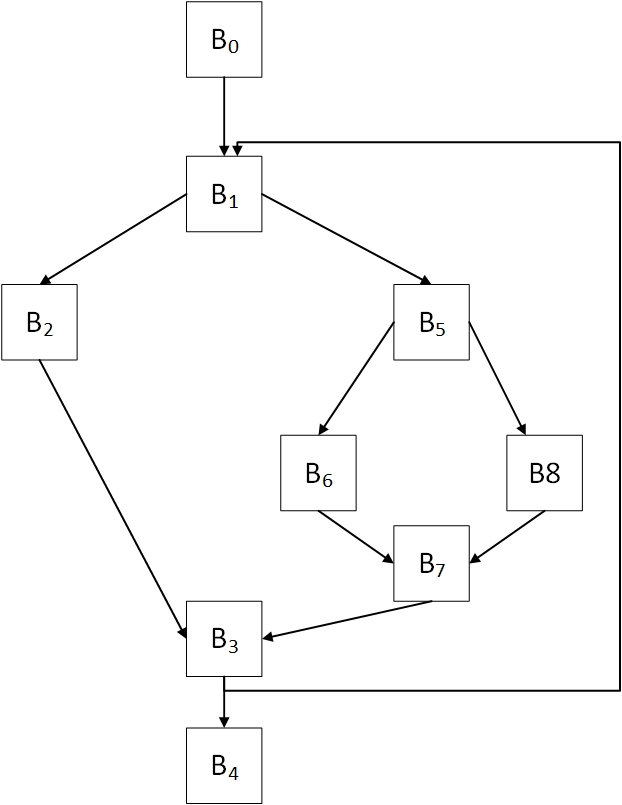
\includegraphics[width=5cm]{./img/figure0.png}
\end{figure}

If we can arrange B5, B6, B8, B7 to be evaluated before B3, we can get more "global" information, i.e., all precursors of B3.

This way we can reduce the number of iterations from 3 to 2

So we need to depth first traverse the entire CFG in reverse post-order \cite{cooper2001simple}
\begin{minted}[mathescape, linenos]{c++}
void Dominators::createReversePostOrder(Function *f) {  // 逆后序
  reversePostOrder_.clear();
  postOrderID_.clear();
  std::set<BasicBlock *> visited;
  postOrderVisit(f->getEntryBlock(), visited);
  reversePostOrder_.reverse();
}

// data structure
class Dominators:{
private:
  std::list<BasicBlock *> reversePostOrder_;
  std::map<BasicBlock *, int> postOrderID_; // the root has highest ID
};

void Dominators::postOrderVisit(BasicBlock *bb, std::set<BasicBlock *> &visited) {
  //从bb开始一趟深度优先遍历
  visited.insert(bb);
  for (auto b : bb->getSuccBasicBlocks()) {
    if (visited.find(b) == visited.end())  // 如果未访问过
      postOrderVisit(b, visited);
  }
  // 节点的后继都访问完毕时
  // 对子节点从深到浅编号
  postOrderID_[bb] = reversePostOrder_.size();
  reversePostOrder_.push_back(bb);
}
\end{minted}
\begin{figure}[htbp]
  \centering
  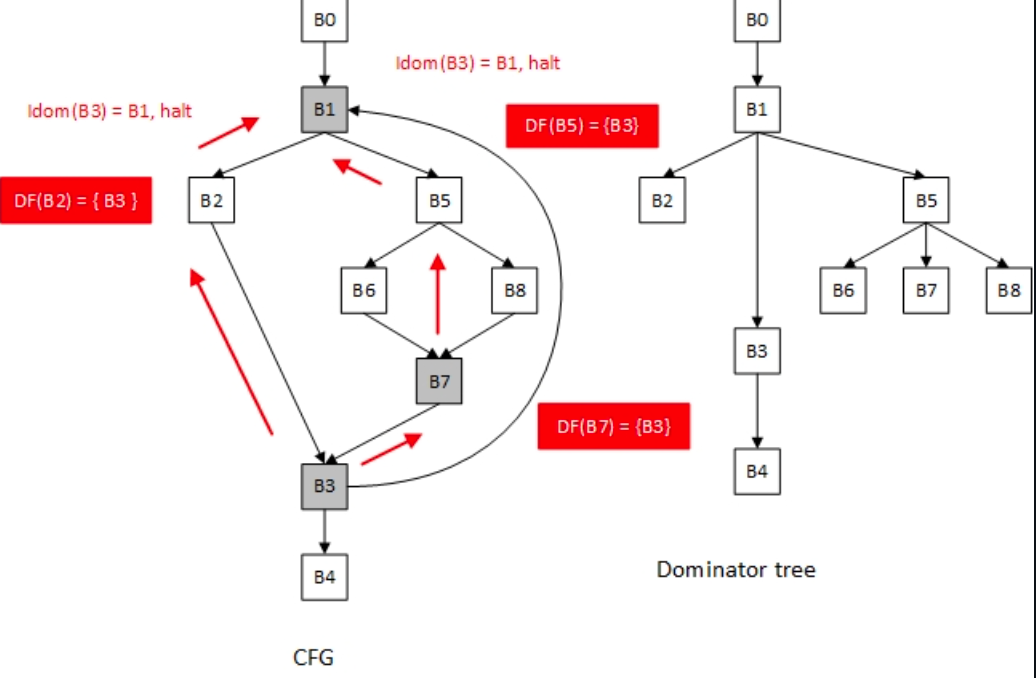
\includegraphics[width=10cm]{./img/figure2.png}
\end{figure}
\end{enumerate}
\subsubsection{InsertPhi}
When generating SSA, it is necessary to calculate where to insert the correct $\phi$. All Basic Blocks with multiple precursors may need to have $\phi$ inserted at the beginning, but this method will insert a lot of useless $\phi$, in order to reduce unnecessary overhead, which BB's need to be inserted at the beginning

For example, in the CFG diagram above, the definition of the variable at B2 does not govern the use of that variable at B3, so the phi instruction needs to be inserted


\subsubsection{SimplifyCFG}
Performs dead code elimination and basic block merging. Specifically:

\begin{enumerate}
  \item Removes basic blocks with no predecessors.
  \item Merges a basic block into its predecessor if there is only one and the predecessor only has one successor.
  \item Eliminates PHI nodes for basic blocks with a single predecessor.
  \item Eliminates a basic block that only contains an unconditional branch.
\end{enumerate}

\begin{minted}[mathescape, linenos]{llvm}
; NOTE: Assertions have been autogenerated by utils/update_test_checks.py
; RUN: opt -instcombine -simplifycfg -S < %s 

target datalayout = "e-m:e-i64:64-f80:128-n8:16:32:64-S128"
target triple = "x86_64-pc-linux-gnu"

; #include <limits>
; #include <cstdint>
;
; using size_type = std::size_t;
; bool will_not_overflow(size_type size, size_type nmemb) {
;   return (size != 0 && (nmemb > std::numeric_limits<size_type>::max() / size));
; }

define i1 @will_not_overflow(i64 %arg, i64 %arg1) {
; SIMPLIFYCFG-LABEL: @will_not_overflow(
;  bb:
;    [[T0:%.*]] = icmp eq i64 [[ARG:%.*]], 0
;    br i1 [[T0]], label [[BB5:%.*]], label [[BB2:%.*]]
;  bb2:
;    [[T3:%.*]] = udiv i64 -1, [[ARG]]
;    [[T4:%.*]] = icmp ult i64 [[T3]], [[ARG1:%.*]]
;    br label [[BB5]]
;  bb5:
;    [[T6:%.*]] = phi i1 [ false, [[BB:%.*]] ], [ [[T4]], [[BB2]] ]
;    ret i1 [[T6]]
;
; INSTCOMBINEONLY-LABEL: @will_not_overflow(
;  bb:
;    [[T0:%.*]] = icmp eq i64 [[ARG:%.*]], 0
;    br i1 [[T0]], label [[BB5:%.*]], label [[BB2:%.*]]
;  bb2:
;    [[UMUL:%.*]] = call { i64, i1 } @llvm.umul.with.overflow.i64(i64 [[ARG]], i64 [[ARG1:%.*]])
;    [[UMUL_OV:%.*]] = extractvalue { i64, i1 } [[UMUL]], 1
;    br label [[BB5]]
;  bb5:
;    [[T6:%.*]] = phi i1 [ false, [[BB:%.*]] ], [ [[UMUL_OV]], [[BB2]] ]
;    ret i1 [[T6]]
;
; INSTCOMBINESIMPLIFYCFGONLY-LABEL: @will_not_overflow(
;  bb:
;    [[T0:%.*]] = icmp eq i64 [[ARG:%.*]], 0
;    [[UMUL:%.*]] = call { i64, i1 } @llvm.umul.with.overflow.i64(i64 [[ARG]], i64 [[ARG1:%.*]])
;    [[UMUL_OV:%.*]] = extractvalue { i64, i1 } [[UMUL]], 1
;    [[T6:%.*]] = select i1 [[T0]], i1 false, i1 [[UMUL_OV]]
;    ret i1 [[T6]]
;
; INSTCOMBINESIMPLIFYCFGINSTCOMBINE-LABEL: @will_not_overflow(
;  bb:
;    [[UMUL:%.*]] = call { i64, i1 } @llvm.umul.with.overflow.i64(i64 [[ARG:%.*]], i64 [[ARG1:%.*]])
;    [[UMUL_OV:%.*]] = extractvalue { i64, i1 } [[UMUL]], 1
;    ret i1 [[UMUL_OV]]
;
; INSTCOMBINESIMPLIFYCFGCOSTLYONLY-LABEL: @will_not_overflow(
;  bb:
;    [[T0:%.*]] = icmp eq i64 [[ARG:%.*]], 0
;    [[UMUL:%.*]] = call { i64, i1 } @llvm.umul.with.overflow.i64(i64 [[ARG]], i64 [[ARG1:%.*]])
;    [[UMUL_OV:%.*]] = extractvalue { i64, i1 } [[UMUL]], 1
;    [[T6:%.*]] = select i1 [[T0]], i1 false, i1 [[UMUL_OV]]
;    ret i1 [[T6]]
;
; INSTCOMBINESIMPLIFYCFGCOSTLYINSTCOMBINE-LABEL: @will_not_overflow(
;  bb:
;    [[UMUL:%.*]] = call { i64, i1 } @llvm.umul.with.overflow.i64(i64 [[ARG:%.*]], i64 [[ARG1:%.*]])
;    [[UMUL_OV:%.*]] = extractvalue { i64, i1 } [[UMUL]], 1
;    ret i1 [[UMUL_OV]]
;
bb:
  %t0 = icmp eq i64 %arg, 0
  br i1 %t0, label %bb5, label %bb2

bb2:                                              ; preds = %bb
  %t3 = udiv i64 -1, %arg
  %t4 = icmp ult i64 %t3, %arg1
  br label %bb5

bb5:                                              ; preds = %bb2, %bb
  %t6 = phi i1 [ false, %bb ], [ %t4, %bb2 ]
  ret i1 %t6
}

; Same as @will_not_overflow, but inverting return value.

define i1 @will_overflow(i64 %arg, i64 %arg1) {
; SIMPLIFYCFG-LABEL: @will_overflow(
;  bb:
;    [[T0:%.*]] = icmp eq i64 [[ARG:%.*]], 0
;    br i1 [[T0]], label [[BB5:%.*]], label [[BB2:%.*]]
;  bb2:
;    [[T3:%.*]] = udiv i64 -1, [[ARG]]
;    [[T4:%.*]] = icmp ult i64 [[T3]], [[ARG1:%.*]]
;    br label [[BB5]]
;  bb5:
;    [[T6:%.*]] = phi i1 [ false, [[BB:%.*]] ], [ [[T4]], [[BB2]] ]
;    [[T7:%.*]] = xor i1 [[T6]], true
;    ret i1 [[T7]]
;
; INSTCOMBINEONLY-LABEL: @will_overflow(
;  bb:
;    [[T0:%.*]] = icmp eq i64 [[ARG:%.*]], 0
;    br i1 [[T0]], label [[BB5:%.*]], label [[BB2:%.*]]
;  bb2:
;    [[UMUL:%.*]] = call { i64, i1 } @llvm.umul.with.overflow.i64(i64 [[ARG]], i64 [[ARG1:%.*]])
;    [[UMUL_OV:%.*]] = extractvalue { i64, i1 } [[UMUL]], 1
;    [[PHITMP:%.*]] = xor i1 [[UMUL_OV]], true
;    br label [[BB5]]
;  bb5:
;    [[T6:%.*]] = phi i1 [ true, [[BB:%.*]] ], [ [[PHITMP]], [[BB2]] ]
;    ret i1 [[T6]]
;
; INSTCOMBINESIMPLIFYCFGONLY-LABEL: @will_overflow(
;  bb:
;    [[T0:%.*]] = icmp eq i64 [[ARG:%.*]], 0
;    [[UMUL:%.*]] = call { i64, i1 } @llvm.umul.with.overflow.i64(i64 [[ARG]], i64 [[ARG1:%.*]])
;    [[UMUL_OV:%.*]] = extractvalue { i64, i1 } [[UMUL]], 1
;    [[PHITMP:%.*]] = xor i1 [[UMUL_OV]], true
;    [[T6:%.*]] = select i1 [[T0]], i1 true, i1 [[PHITMP]]
;    ret i1 [[T6]]
;
; INSTCOMBINESIMPLIFYCFGINSTCOMBINE-LABEL: @will_overflow(
;  bb:
;    [[UMUL:%.*]] = call { i64, i1 } @llvm.umul.with.overflow.i64(i64 [[ARG:%.*]], i64 [[ARG1:%.*]])
;    [[UMUL_OV:%.*]] = extractvalue { i64, i1 } [[UMUL]], 1
;    [[PHITMP:%.*]] = xor i1 [[UMUL_OV]], true
;    ret i1 [[PHITMP]]
;
; INSTCOMBINESIMPLIFYCFGCOSTLYONLY-LABEL: @will_overflow(
;  bb:
;    [[T0:%.*]] = icmp eq i64 [[ARG:%.*]], 0
;    [[UMUL:%.*]] = call { i64, i1 } @llvm.umul.with.overflow.i64(i64 [[ARG]], i64 [[ARG1:%.*]])
;    [[UMUL_OV:%.*]] = extractvalue { i64, i1 } [[UMUL]], 1
;    [[PHITMP:%.*]] = xor i1 [[UMUL_OV]], true
;    [[T6:%.*]] = select i1 [[T0]], i1 true, i1 [[PHITMP]]
;    ret i1 [[T6]]
;
; INSTCOMBINESIMPLIFYCFGCOSTLYINSTCOMBINE-LABEL: @will_overflow(
;  bb:
;    [[UMUL:%.*]] = call { i64, i1 } @llvm.umul.with.overflow.i64(i64 [[ARG:%.*]], i64 [[ARG1:%.*]])
;    [[UMUL_OV:%.*]] = extractvalue { i64, i1 } [[UMUL]], 1
;    [[PHITMP:%.*]] = xor i1 [[UMUL_OV]], true
;    ret i1 [[PHITMP]]
;
bb:
  %t0 = icmp eq i64 %arg, 0
  br i1 %t0, label %bb5, label %bb2

bb2:                                              ; preds = %bb
  %t3 = udiv i64 -1, %arg
  %t4 = icmp ult i64 %t3, %arg1
  br label %bb5

bb5:                                              ; preds = %bb2, %bb
  %t6 = phi i1 [ false, %bb ], [ %t4, %bb2 ]
  %t7 = xor i1 %t6, true
  ret i1 %t7
}
\end{minted}

\printbibliography
\end{document}
